\section{Non-crossing 2-partitions}

\begin{definition}[Non-crossing 2-partition]
    A \emph{non-crossing 2-partition} of a \emph{totally
    ordered} set $E$ is a pair $(P, \sigma)$
    where :\\
    \begin{itemize*}
        \item $P$ is a non-crossing partition of $E$\\
        \item $\sigma$ is a permutation of the elements of $E$\\
        \item For each \emph{sorted} block
            $B_i = \{b_1, \ldots, b_k\} \in P$, we have
            $\sigma (b_i) < \ldots < \sigma (b_k)$\\\\
    \end{itemize*}
    We denote by $\mathcal{NC}^2_n$ the set of non-crossing
    2-partitions of $[n]$.
    $$\mathcal{NC}^2 = \bigcup_{n > 0}{\mathcal{NC}^2_n}$$.
\end{definition}

\begin{example}[$\mathcal{NC}^2_6$]
    \begin{itemize*}
            \subitem $P = \{\{1, 6\}, \{2, 3, 5\}, \{4\}\}$
            \subitem $\sigma = 413265$ \\
            \subitem $\hspace{36mm} \rho = \{\{1, 3, 6\}, \{2\}, \{4, 5\}\}$
    \end{itemize*}    
\end{example}

\begin{theorem}
    Let $nc^2_n$ be the cardinal of $\mathcal{NC}^2_n$.
    We have $$nc^2_n = (n + 1)^{n-1}$$
\end{theorem}

\begin{example}[$n = 1, 2, 3$]
    ~\\
    \begin{itemize}
            \item $n = 1$ \  $:$ \  $nc^2_1 = 1$
            \subitem $\{\{1\}\}$ \hspace{1cm} $1$
                \hspace{1cm} $\rho = P$
            \item $n = 2$ \  $:$ \  $nc^2_2 = 3$
            \subitem $\{\{1\}, \{2\}\}$ \hspace{1cm} $12$
                \hspace{1cm} $\rho = P$
            \subitem $\{\{1\}, \{2\}\}$ \hspace{1cm} $21$
                \hspace{1cm} $\rho = P$
            \subitem $\{\{1, 2\}\}$ \hspace{14mm} $12$
                \hspace{1cm} $\rho = P$
            \item $n = 3$ \  $:$ \  $nc^2_3 = 16$
            \subitem $\{\{1\}, \{2\}, \{3\}\}$ \hspace{1cm}
                $123$ \hspace{1cm} $\rho = P$
            \subitem $\{\{1\}, \{2\}, \{3\}\}$ \hspace{1cm}
                $132$ \hspace{1cm} $\rho = P$
            \subitem $\{\{1\}, \{2\}, \{3\}\}$ \hspace{1cm}
                $213$ \hspace{1cm} $\rho = P$
            \subitem $\{\{1\}, \{2\}, \{3\}\}$ \hspace{1cm}
                $231$ \hspace{1cm} $\rho = P$
            \subitem $\{\{1\}, \{2\}, \{3\}\}$ \hspace{1cm}
                $312$ \hspace{1cm} $\rho = P$
            \subitem $\{\{1\}, \{2\}, \{3\}\}$ \hspace{1cm}
                $321$ \hspace{1cm} $\rho = P$       
            \subitem $\{\{1, 2\}, \{3\}\}$ \hspace{14mm}
                $123$ \hspace{1cm} $\rho = P$
            \subitem $\{\{1, 2\}, \{3\}\}$ \hspace{14mm}
                $132$ \hspace{1cm} $\rho = \{\{1, 3\}, \{2\}\}$
            \subitem $\{\{1, 2\}, \{3\}\}$ \hspace{14mm}
                $231$ \hspace{1cm} $\rho = \{\{1\}, \{2, 3\}\}$
            \subitem $\{\{1\}, \{2, 3\}\}$ \hspace{14mm}
                $123$ \hspace{1cm} $\rho = P$
            \subitem $\{\{1\}, \{2, 3\}\}$ \hspace{14mm}
                $213$ \hspace{1cm} $\rho = \{\{1, 3\}, \{2\}\}$
            \subitem $\{\{1\}, \{2, 3\}\}$ \hspace{14mm}
                $312$ \hspace{1cm} $\rho = \{\{1, 2\}, \{3\}\}$
            \subitem $\{\{1, 3\}, \{2\}\}$ \hspace{14mm}
                $123$ \hspace{1cm} $\rho = P$
            \subitem $\{\{1, 3\}, \{2\}\}$ \hspace{14mm}
                $132$ \hspace{1cm} $\rho = \{\{1, 2\}, \{3\}\}$
            \subitem $\{\{1, 3\}, \{2\}\}$ \hspace{14mm}
                $213$ \hspace{1cm} $\rho = \{\{1\}, \{2, 3\}\}$  
            \subitem $\{\{1, 2, 3\}\}$ \hspace{18mm}
                $123$ \hspace{1cm} $\rho = P$\\
    \end{itemize}
\end{example}

\begin{prop}
    This means we can create a \emph{bijection} between
    $\mathcal{PF}_n$ and $\mathcal{NC}^2_n$.
\end{prop}

\begin{proof}
    ~\\
\begin{itemize}
    \item $\mathcal{PF}_n \to \mathcal{NC}^2_n$ :
    Let $f = (a_1, \ldots, a_n) \in \mathcal{PF}_n$
    be our parking function.
    For $i \in \{1, \ldots, n\}$, we define :
        \subitem $l_i$ : the number of occurences of $i$ in $f$. 
        \subitem $im_i$ : $\{j\ |\ a_j = i\}$\\
    The corresponding non-crossing partition will
    have the following constraints :
        \subitem For each $i \in \{1, \ldots, n\}$, if $l_i > 0$,
        then there is a block $B_{[i]}$ of length
        \subitem $l_i$ with minimum element $i$.
        \subitem $\sigma (B_{[i]}) = im_i$\\
    There is a unique set partition
    $\displaystyle P = \bigcup_{i}{B}_{[i]}$ of $[n]$
    and a unique permutation $\sigma$ respecting these
    conditions such that $(P, \sigma) \in \mathcal{NC}^2_n$ :
    for each minimum $i$ in \emph{decreasing order}, add
    the $n_i$ first free elements of
    $[i+1, i+2, \ldots, n, 1, \ldots, i-1]$ to $B_i$.
    $\sigma$ is then trivially obtained by the second
    constraint. 
    \item $\mathcal{NC}^2_n \to \mathcal{PF}_n$ :
    Let $(P, \sigma)$ with $P = \{B_1, \ldots, B_l\}$ be our
    non-crossing 2-partition.
    For each block $B_i = \{b_1, \ldots, b_k\} \in P$ :
    \subitem $m_i = min (B_i) = b_1$
    \subitem $pos_i = \sigma (B_i)$
    \subitem For each $j \in pos_i$, we define $a_j = m_i$\\
    The corresponding parking function is $(a_1, \ldots, a_n)$.
\end{itemize}
\end{proof}

\begin{example}[$n = 8$]
    \begin{align*}
        &P = \{\{1, 2, 5\}, \{3, 4\}, \{6, 8\}, \{7\}\}\\
        &\sigma = 36187245\\
        &f = (3, 6, 1, 7, 6, 1, 1, 3)\\
    \end{align*}
\end{example}

\subsection{The non-crossing 2-partitions poset}

\begin{definition}[$\succ^2$]
    We say that $(P, \sigma)$ covers $(Q, \tau)$, written
    ($P, \sigma) \succ^2 (Q, \tau)$,
    if $\exists B_i, B_j \in P$ such that\\
    \begin{itemize*}
        \item $Q = P - \{B_i, B_j\} \cup \{B_i \cup B_j\}$\\
        \item $l \neq i, j \and b \in B_l \rightarrow
            \tau (b) = \sigma (b)$\\
        \item Let $B_i \cup B_j = \{b_1, \ldots, b_k\}$ :\\
            \subitem $\tau (B_i \cup B_j) = \sigma (B_i \cup B_j)$\\
            \subitem $\tau (b_1) < \ldots < \tau (b_k)$
    \end{itemize*}    
\end{definition}

\begin{example}
    ~\\
    \begin{itemize*}
        \item $P = \{\{1, 6\}, \{2, 3\}, \{4\}, \{5\}\}$\\
        \item $\sigma = 236154$\\
        \item $Q = \{\{1, 6\}, \{2, 3, 5\}, \{4\}\}$\\
        \item $\tau = 235164$\\
        \item $(P, \sigma) \succ^2 (Q, \tau)$\\
        \item $(P, \sigma) \not \succ^2 (Q, \sigma)$,
        because  $\sigma (\{2, 3, 5\}) = \{3, 6, 5\}$ is
        \emph{not} ordemagenta. 
    \end{itemize*}
\end{example}

\begin{prop}
    This covering relation defines the \emph{poset} of
    $\mathcal{NC}^2_n$.
\end{prop}

\begin{rem}
    The bottom element of this poset is 
    $(\{\{1, \ldots, n\}\}, 12 \ldots n)$, and the top
    elements are $\{(\{\{1\}, \ldots, \{n\}\}, \sigma)\ 
    |\ \sigma \in \mathfrak{S}_n\}$.
\end{rem}

\begin{example}[The poset of $\mathcal{NC}^2_3$]
    ~\\
    To shorten labels, we represent
    $(\{\{1, 3\}, \{2\}\}, 213)$ by \\
    \begin{center}
        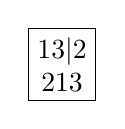
\begin{tikzpicture}
            \node (0) at (0,0) [align = center]
            [rectangle, draw]{$13|2$\\$213$};
        \end{tikzpicture}
    \end{center}

    \begin{center}
        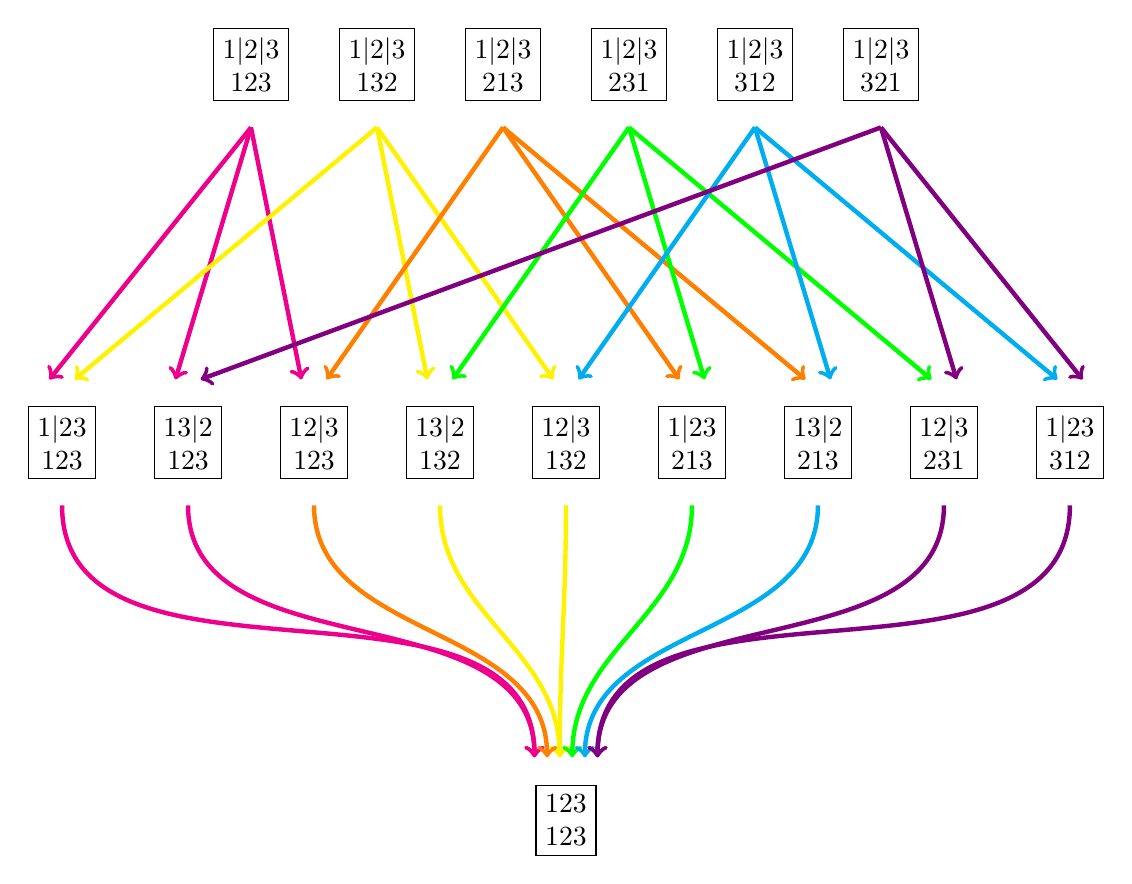
\begin{tikzpicture}[scale = 0.8]
            \node (0)  at (0,0) [align = center]
            [rectangle, draw]
                {$123$\\$123$};
            \node (1)  at (-8,6)[align = center]
            [rectangle, draw]
                {$1|23$\\$123$};
            \node (2)  at (-6,6) [align = center]
            [rectangle, draw]
                {$13|2$\\$123$};
            \node (3)  at (-4,6) [align = center]
            [rectangle, draw]
                {$12|3$\\$123$};
            \node (4)  at (-2,6) [align = center]
            [rectangle, draw]
                {$13|2$\\$132$};
            \node (5)  at (0,6) [align = center]
            [rectangle, draw]
                {$12|3$\\$132$};
            \node (6)  at (2,6) [align = center]
            [rectangle, draw]
                {$1|23$\\$213$};
            \node (7)  at (4,6) [align = center]
            [rectangle, draw]
                {$13|2$\\$213$};
            \node (8)  at (6,6) [align = center]
            [rectangle, draw]
                {$12|3$\\$231$};
            \node (9)  at (8,6) [align = center]
            [rectangle, draw]
                {$1|23$\\$312$};
            \node (10) at (-5,12) [align = center]
            [rectangle, draw]
                {$1|2|3$\\$123$};
            \node (11) at (-3,12) [align = center]
            [rectangle, draw]
                {$1|2|3$\\$132$};
            \node (12) at (-1,12) [align = center]
            [rectangle, draw]
                {$1|2|3$\\$213$};
            \node (13) at (1,12) [align = center]
            [rectangle, draw]
                {$1|2|3$\\$231$};
            \node (14) at (3,12) [align = center]
            [rectangle, draw]
                {$1|2|3$\\$312$};
            \node (15) at (5,12) [align = center]
            [rectangle, draw]
                {$1|2|3$\\$321$};
        
            \draw [->][color=magenta, ultra thick]
                (-5,11) to (-8.2,7);
            \draw [->][color=magenta, ultra thick]
                (-5,11) to (-6.2, 7); 
            \draw [->][color=magenta, ultra thick]
                (-5,11) to (-4.2,7);
            \draw [->][out=-90,in=90, ultra thick] 
                [color=magenta](-8,5) to (-0.5,1);
            \draw [->][out=-90,in=90, ultra thick] 
                [color=magenta](-6,5) to (-0.5,1);
        
            \draw [->][color=yellow, ultra thick]
                (-3,11) to (-7.8,7);
            \draw [->][color=yellow, ultra thick]
                (-3,11) to (-2.2,7);
            \draw [->][color=yellow, ultra thick]
                (-3,11) to (-0.2, 7);
            \draw [->][out=-90,in=90, ultra thick] 
                [color=yellow](-2,5) to (-0.1,1);
            \draw [->][out=-90,in=90, ultra thick] 
                [color=yellow](0,5) to (-0.1,1);
            
            \draw [->][color=orange, ultra thick]
                (-1,11) to (1.8,7);
            \draw [->][color=orange, ultra thick]
                (-1,11) to (3.8,7);
            \draw [->][color=orange, ultra thick]
                (-1,11) to (-3.8,7);
            \draw [->][out=-90,in=90, ultra thick] 
                [color=orange](-4,5) to (-0.3,1);
        
            \draw [->][color=green, ultra thick]
                (1,11) to (2.2,7);
            \draw [->][color=green, ultra thick]
                (1,11) to (-1.8,7);
            \draw [->][color=green, ultra thick]
                (1,11) to (5.8,7);
            \draw [->][out=-90,in=90, ultra thick] 
                [color=green](2,5) to (0.1,1);
        
            \draw [->][color=cyan, ultra thick]
                (3,11) to (7.8,7);
            \draw [->][color=cyan, ultra thick]
                (3,11) to (4.2,7);
            \draw [->][color=cyan, ultra thick]
                (3,11) to (0.2,7);
            \draw [->][out=-90,in=90, ultra thick] 
                [color=cyan](4,5) to (0.3,1);
        
            \draw [->][color=violet, ultra thick]
                (5,11) to (8.2,7);
            \draw [->][color=violet, ultra thick]
                (5,11) to (-5.8,7);
            \draw [->][color=violet, ultra thick]
                (5,11) to (6.2,7);
            \draw [->][out=-90,in=90, ultra thick] 
                [color=violet](6,5) to (0.5,1);
            \draw [->][out=-90,in=90, ultra thick] 
                [color=violet](8,5) to (0.5,1);
            
        \end{tikzpicture}
        ~\\
        There are $4^2 = 16$ elements in this poset.
    \end{center}
\end{example}

\subsection{The parking functions poset}

\begin{definition}[Rank]
    Given $f = (a_1, \ldots, a_n) \in \mathcal{PF}_n$, let
    $$b_i =
    \begin{cases}
        1 \text{ if } \exists j\ |\ a_j = i\\
        0 \text{ otherwise}
    \end{cases} $$
    We define the \emph{rank} of $f$, noted $rk(f)$, as
    $$\sum_{1 \leq i \leq n}{b_i}$$
\end{definition}

\begin{example}
    \begin{align*}
        &rk((1, 5, 4, 2, 3, 3, 1)) = 5\\
        &rk((4, 7, 1, 1, 3, 2 ,2, 8)) = 6\\
    \end{align*}
\end{example}

\begin{definition}[$\succ_{pf}$]
    Since $\mathcal{PF}_n$ and $\mathcal{NC}^2_n$ are
    in bijection, we can define a \emph{covering relation}
    $\succ_{pf}$ for $\mathcal{PF}_n$ as follows :\\
    $f \in \mathcal{PF}_n \succ_{pf} g \in \mathcal{PF}_n$
    if and only if :    
    \begin{itemize}
        \item $(P,\sigma)$ is the non-crossing 2-partition
        associated to $f$
        \item $(Q, \tau)$ is the non-crossing 2-partition
        associated to $g$
        \item $(P, \sigma) \succ^2 (Q, \tau)$
    \end{itemize}
\end{definition}

\begin{example}
    ~\\
    \begin{itemize*}
        \item $P = \{\{1, 6\}, \{2, 3\}, \{4\}, \{5\}\}$\\
        \item $\sigma = 236154$\\
        \item $Q = \{\{1, 6\}, \{2, 3, 5\}, \{4\}\}$\\
        \item $\tau = 235164$\\
        \item $f = (4, 1, 2, 1, 5, 2) \succ_{pf}
            g = (4, 1, 2, 1, 2, 2)$\\
    \end{itemize*}
\end{example}

\begin{rem}
    If $f \succ_{pf} g$, then $rk(f) = rk(g) + 1$, and
    there exists $i$ and $j$ such that :
    \begin{itemize}
        \item $i < j$
        \item There is at least $1$ occurence of $i$ in $f$
        \item There is at least $1$ occurence of $j$ in $f$
        $$b_k =
            \begin{cases}
                i \text{ if } a_k = j\\
                a_k \text{ otherwise}\\
            \end{cases}$$
    \end{itemize}
\end{rem}

\begin{prop}
    This covering relation defines the \emph{poset}
    of $\mathcal{PF}_n$.
\end{prop}

\begin{rem}
    The bottom element of this poset is
    $(\underbrace{1, \ldots, 1}_{n})$,
    and the top elements are the \emph{permutations} of
    $\{1, \ldots, n\}$.
\end{rem}

\begin{example}[The poset of $\mathcal{PF}_3$]
    ~\\
    \begin{center}
        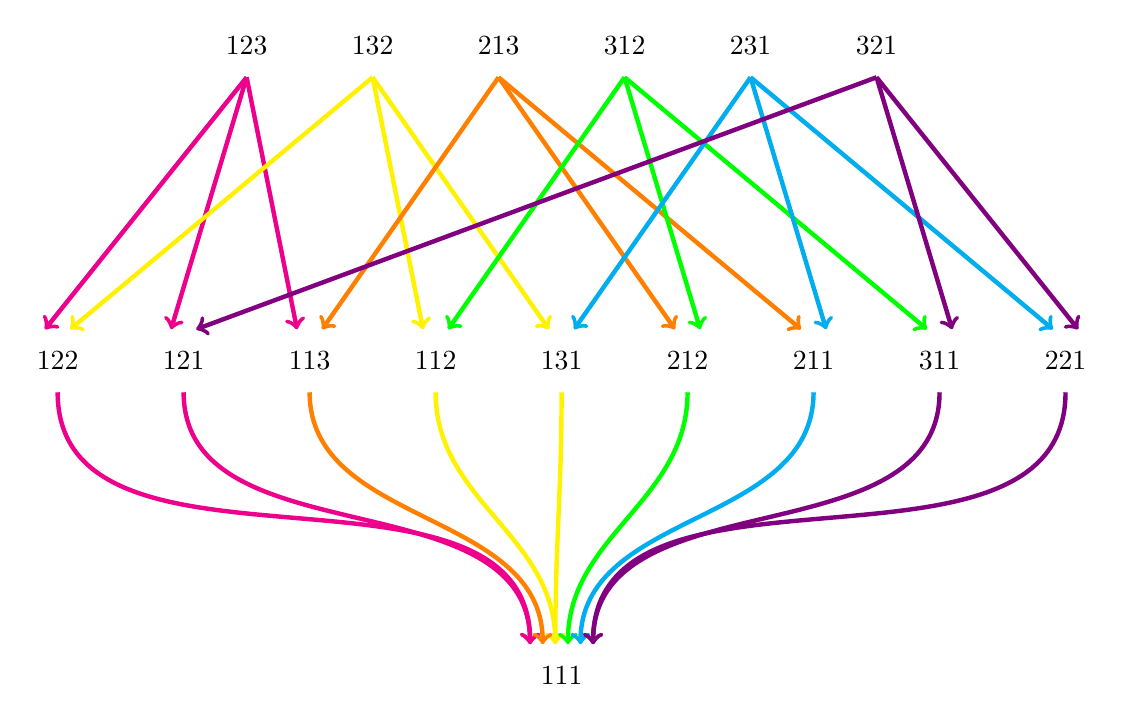
\begin{tikzpicture}[scale = 0.8]
            \node (0)  at (0,0)   {$111$};
            \node (1)  at (-8,5)  {$122$};
            \node (2)  at (-6,5)  {$121$};
            \node (3)  at (-4,5)  {$113$};
            \node (4)  at (-2,5)  {$112$};
            \node (5)  at (0,5)   {$131$};
            \node (6)  at (2,5)   {$212$};
            \node (7)  at (4,5)   {$211$};
            \node (8)  at (6,5)   {$311$};
            \node (9)  at (8,5)   {$221$};
            \node (10) at (-5,10) {$123$};
            \node (11) at (-3,10) {$132$};
            \node (12) at (-1,10) {$213$};
            \node (13) at (1,10)  {$312$};
            \node (14) at (3,10)  {$231$};
            \node (15) at (5,10)  {$321$};
        
            \draw [->][color=magenta, ultra thick]
                (-5,9.5) to (-8.2,5.5);
            \draw [->][color=magenta, ultra thick]
                (-5,9.5) to (-6.2,5.5); 
            \draw [->][color=magenta, ultra thick]
                (-5,9.5) to (-4.2,5.5);
            \draw [->][out=-90,in=90, ultra thick] 
                [color=magenta](-8,4.5) to (-0.5,0.5);
            \draw [->][out=-90,in=90, ultra thick] 
                [color=magenta](-6,4.5) to (-0.5,0.5);
        
            \draw [->][color=yellow, ultra thick]
                (-3,9.5) to (-7.8,5.5);
            \draw [->][color=yellow, ultra thick]
                (-3,9.5) to (-2.2,5.5);
            \draw [->][color=yellow, ultra thick]
                (-3,9.5) to (-0.2,5.5);
            \draw [->][out=-90,in=90, ultra thick] 
                [color=yellow](-2,4.5) to (-0.1,0.5);
            \draw [->][out=-90,in=90, ultra thick] 
                [color=yellow](0,4.5) to (-0.1,0.5);
            
            \draw [->][color=orange, ultra thick]
                (-1,9.5) to (1.8,5.5);
            \draw [->][color=orange, ultra thick]
                (-1,9.5) to (3.8,5.5);
            \draw [->][color=orange, ultra thick]
                (-1,9.5) to (-3.8,5.5);
            \draw [->][out=-90,in=90, ultra thick] 
                [color=orange](-4,4.5) to (-0.3,0.5);
        
            \draw [->][color=green, ultra thick]
                (1,9.5) to (2.2,5.5);
            \draw [->][color=green, ultra thick]
                (1,9.5) to (-1.8,5.5);
            \draw [->][color=green, ultra thick]
                (1,9.5) to (5.8,5.5);
            \draw [->][out=-90,in=90, ultra thick] 
                [color=green](2,4.5) to (0.1,0.5);
        
            \draw [->][color=cyan, ultra thick]
                (3,9.5) to (7.8,5.5);
            \draw [->][color=cyan, ultra thick]
                (3,9.5) to (4.2,5.5);
            \draw [->][color=cyan, ultra thick]
                (3,9.5) to (0.2,5.5);
            \draw [->][out=-90,in=90, ultra thick] 
                [color=cyan](4,4.5) to (0.3,0.5);
        
            \draw [->][color=violet, ultra thick]
                (5,9.5) to (8.2,5.5);
            \draw [->][color=violet, ultra thick]
                (5,9.5) to (-5.8,5.5);
            \draw [->][color=violet, ultra thick]
                (5,9.5) to (6.2,5.5);
            \draw [->][out=-90,in=90, ultra thick] 
                [color=violet](6,4.5) to (0.5,0.5);
            \draw [->][out=-90,in=90, ultra thick] 
                [color=violet](8,4.5) to (0.5,0.5);
            
        \end{tikzpicture}
    \end{center}
\end{example}